\documentclass[plainboxedsections, 17pt, b1]{sciposter}
%\documentclass[plainboxedsections, 17pt, b1,draft]{sciposter}
\renewcommand{\titlesize}{\Huge}


\usepackage[polish]{babel}
\usepackage[utf8]{inputenc}
%\usepackage[cp1250]{inputenc}
\usepackage[T1]{fontenc}

\usepackage{fancybox}
\usepackage{multicol}
\usepackage{sectionbox}

\usepackage{fancyhdr}
%\usepackage{dsfont}
\usepackage{graphicx}
\usepackage{subfig}
\usepackage{amsmath}
\addto\captionspolish{\renewcommand{\figurename}{Figure}}

\leftlogo[1]{ccfd3.png}
\rightlogo[1]{logo_PW.png}
\title{Residual Distribution Method for~unsteady Euler~equations}
\author{Marcin Wyrozębski}
\institute{Department of Aerodynamics\\
Institute of Aeronautics and Applied Mechanics \\
Warsaw University of Technology 
}
\email{mwyrozebski@meil.pw.edu.pl}


\definecolor{mainCol}{RGB}{255,255,255} %dark blue
%\definecolor{TextCol}{rgb}{1.0,1.0,0.5} %white
\definecolor{SectionCol}{RGB}{255,255,255} %orange
\definecolor{BoxCol}{RGB}{43, 90, 112} %white

%\definecolor{sectboxrulecol}{%rgb}{0,0,0.5}

\definecolor{sectboxfillcol}{RGB}{230,230,230} 
\definecolor{sectboxrulecol}{RGB}{224,224,224}  
%\definecolor{sectboxtextcol}{%rgb}{0,0,1}
%\definecolor{subsectboxrulecol}{%rgb}{0,0.5,0}
%\definecolor{subsectboxfillcol}{%rgb}{0.9,1,0.9}
%\definecolor{subsectboxtextcol}{%rgb}{0,1,0}
%\definecolor{subsubsectboxrulecol}{%rgb}{0.5,0,0}
%\definecolor{subsubsectboxfillcol}{%rgb}{1,0.9,0.9}
%\definecolor{subsubsectboxtextcol}{%rgb}{1,0,0}


\renewcommand{\headrulewidth}{0pt}

\newcommand{\fracpd}[2]{\frac{\partial #1}{\partial #2}}
\newcommand{\rd}{$\mathcal{RD}$}

\begin{document}
%\lfoot{
\includegraphics[width=0.16\textwidth]{pokl.png}}
\cfoot{{\bf KKMP 2014}, XXI Fluid Mechanics Conference, Krakow, Poland }
%\rfoot{
\includegraphics[width=0.16\textwidth]{ue.png}}
%\setlength{\footskip}{3cm}
\pagestyle{fancy}

\maketitle

%\begin{abstract}
%optional abstract
%\end{abstract}

\section{Introduction }

Partial Differential Equations (PDEs) plays significant role in modelling many physical phenomenons. As there are no analytical method to solve such problems in general, numerical methods are applied to obtained approximate solution. Presented here Residual Distribution (\rd{}) Method (called also Fluctuation Splitting) has few important advantages over commonly used Finite Volume Method (FVM) and Finite Element Method (FEM) which motivates our investigation on that topic. In order to satisfy monotonicity condition FEM uses additional shock capturing terms, which has some adjustable parameters hard to define in general way. On the other hand second order FVM requires data from neighbour which causes some problems with parallel implementation. \rd{} method allows to solve general partial differential equations even highly nonlinear in an accurate, robust and efficient manner.


\begin{multicols}{3}

% #################################################
\section{Residual Distribution Method}
% #################################################
	Main advantages of Residual Distribution (\rd{}) Method are
	\begin{itemize}
		\item True multidimensional upwind in 2D and 3D
		\item Monotone, parameter free capturing solution discontinuities
		\item Compact nearest-neighbour stencil 
		\item Application for shallow-water, multiphase and MHD equations
		\item Ease of including source terms
		\item Application for triangular and quadrilateral elements
	\end{itemize}
\vspace{.3cm}

	\rd{} procedure for general steady hyperbolic equation:
	\[ \fracpd{u}{t} + \nabla \cdot \mathcal{F}(u) = 0 \]
	\begin{enumerate}
		\item For each element in mesh compute fluctuation
			\[ \phi^E = \int_E \nabla \cdot F(u) \, d E \]
		\item For each element in mesh split fluctuation between nodes using specified scheme
			\[ \phi_i = \beta_i \phi^E \]
		\item For each node aggregate fluctation signals from whole mesh and update solution
			\[ u_i^{n+1} = u_i^n + c_i \sum_j \phi_j 	\]
	\end{enumerate}
Fluctuation splitting can be done in numerous ways, so in fact \rd{} is a~group of schemes which differs in that step and so have different properties.

% #################################################
\section{Steady advection equation}
% #################################################
	Steady advection equation can be written in form
		\[ \fracpd{u}{t} + \nabla \cdot \mathcal{F}(u) = 0 , \quad \mathcal{F}(u) = \lambda u, \quad \lambda = ( \lambda_x , \lambda_y ) \]
	%\[ \fracpd{u}{t} + \lambda \cdot \nabla u = 0 \]
	
	Including some preliminary definitions:
	\begin{itemize}
		\item normal vector to node -- oriented to interior of element, has length of edge opposite to node\\
	\end{itemize}
		\[ n_i = (y_j-y_k) e_x + (x_j-x_k)  e_y  \]
		\begin{figure}%
			\centering
			\def\svgwidth{0.3\columnwidth}
			\input{img/trojkatnorm.pdf_tex}
			\caption{Set of normal vectors for a triangular element}
		\end{figure}
		\begin{itemize}
			\item inflow parameter -- advection velocity vector $\lambda$ projected on normal vector $n_i$
		\end{itemize}
			\[ k_i = \lambda \cdot n_i \]
	and assuming linear change of $u$ in element $E$ fluctuation $\phi^E$ can be written in closed formula:
	\[ \phi^E = \int_E \nabla \cdot \mathcal{F}(u) = \int_E \lambda \cdot \nabla u = \sum_{i=1}^3 k_i u_i 	\]
	
	Fluctuation splitting step has the biggest influence on the properties of method, for that reason \rd{} schemes can be divided in two groups presented below with the most accurate scheme from each group:
	\begin{itemize}
		\item linear schemes - distribution to nodes does not depend on the solution
			\begin{itemize}
				\item monotone: Narrow (N)
				\item second order: Low Diffusion A (LDA)
			\end{itemize}
		\item nonlinear schemes
			\begin{itemize}
				\item blended: LDA-N
				\item limited: Limited N (LimN)
			\end{itemize}
	\end{itemize}
	
	Due to Godunov's theorem only nonlinear schemes can achieve second order of accuracy meeting monotonicity condition at the same time. 
	
\section{Unsteady equations}
	Considering \rd{} formulation for unsteady equations the procedure in general stays the same like in steady cases. 
	Main difference is that time derivative must be taken into account when computing fluctuation, but still it can be written in closed form with modified inflow parameters $k_i$:
	\[ \phi^E = \int_{t^n}^{t^{n+1}} \int_E \left( \fracpd{u}{t} + \nabla \cdot \mathcal{F}(u) \right) = \sum_{i=1}^3 k_i u_i \]


% #################################################
\section{Results}
% #################################################

\begin{enumerate}
	\item \textbf{Unsteady advection equation}
		\[ \fracpd{u}{t} + \lambda \cdot \nabla u = 0, \quad \lambda = ( \, 0.5 \, , \, 0.25 \,  ) \]
\end{enumerate}
This test case considers linear advection with constant velocity. Initial solution has smooth cosine hill shape. Results for two schemes (N and LDA) and section along $y=0$ line are presented below. It can be seen that LDA schemes offers great accuracy, but some oscilations occurs. On the other hand, N scheme satisfies monotonicity condition, but is much more dissipative.

\begin{figure}%
	\centering
	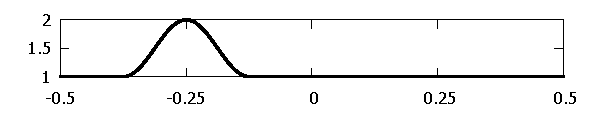
\includegraphics[width=0.45\columnwidth]{img/advect_initial_cosine.pdf} \\
	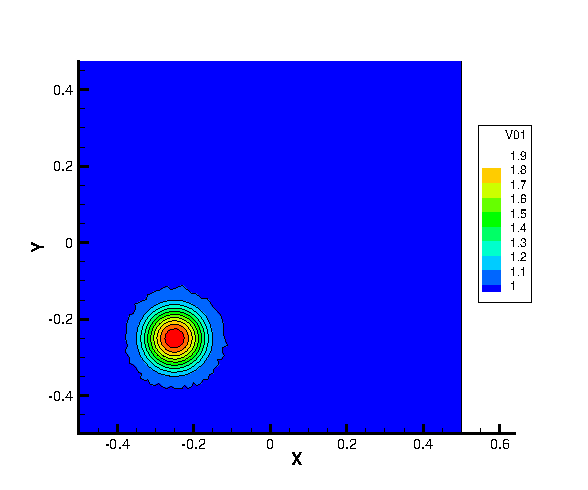
\includegraphics[width=0.45\columnwidth]{img/advect_initial_cosine_map.pdf}%
	\caption{Advection -- initial solution map and section }%
\end{figure}

\begin{figure}%
	\centering
	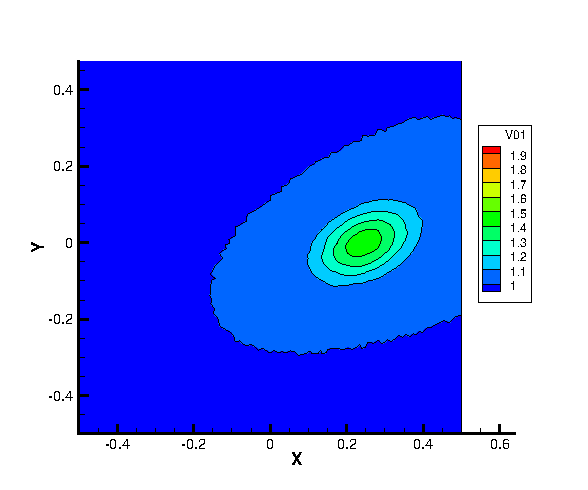
\includegraphics[width=0.45\columnwidth]{img/advect_lin_n_map.pdf} 
	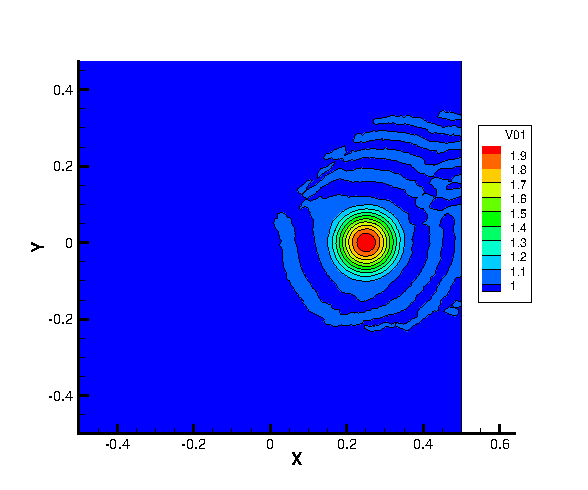
\includegraphics[width=0.45\columnwidth]{img/advect_lin_lda_map.pdf} \\
	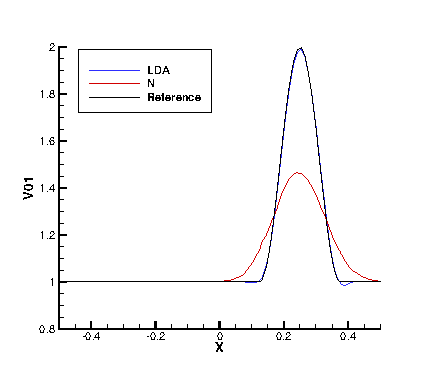
\includegraphics[width=0.45\columnwidth]{img/advect_lin_section.pdf}%
	\caption{Advection -- final solution for N (left) and LDA (right) schemes and section at $y=0$ (bottom)}%
\end{figure}
		

\begin{enumerate}\addtocounter{enumi}{1}
	\item \textbf{Unsteady Euler equations}
\end{enumerate}
\[ \fracpd{u}{t} + \nabla \cdot \mathcal{F}(u) = 0, \quad u = \left( \begin{array}{c} \rho \\ \rho u \\ \rho v \\ \rho E \end{array} \right), \quad  \mathcal{F} (u) = \left( 
			\begin{array}{cc}	\rho u & \rho v \\ \rho u^2 + p & \rho u v \\ \rho u v & \rho v^2 + p \\ \rho H u & \rho H v \end{array} \right) \]

\begin{enumerate}\addtocounter{enumi}{1}
	\item \begin{enumerate}
		\item \textbf{2D Riemann case}:
	\end{enumerate}
\end{enumerate}
This case is focused on solving initial Riemann problem in 2 dimensions. Initial solution has checkerboard pattern with regions of high and low density and pressure. Two schemes were considered: N and LimN. As can be seen on contour maps and section plot, the latter provides much better resolution of discontinuities satisfying monotonicity condition.

\begin{figure}%
	\centering
	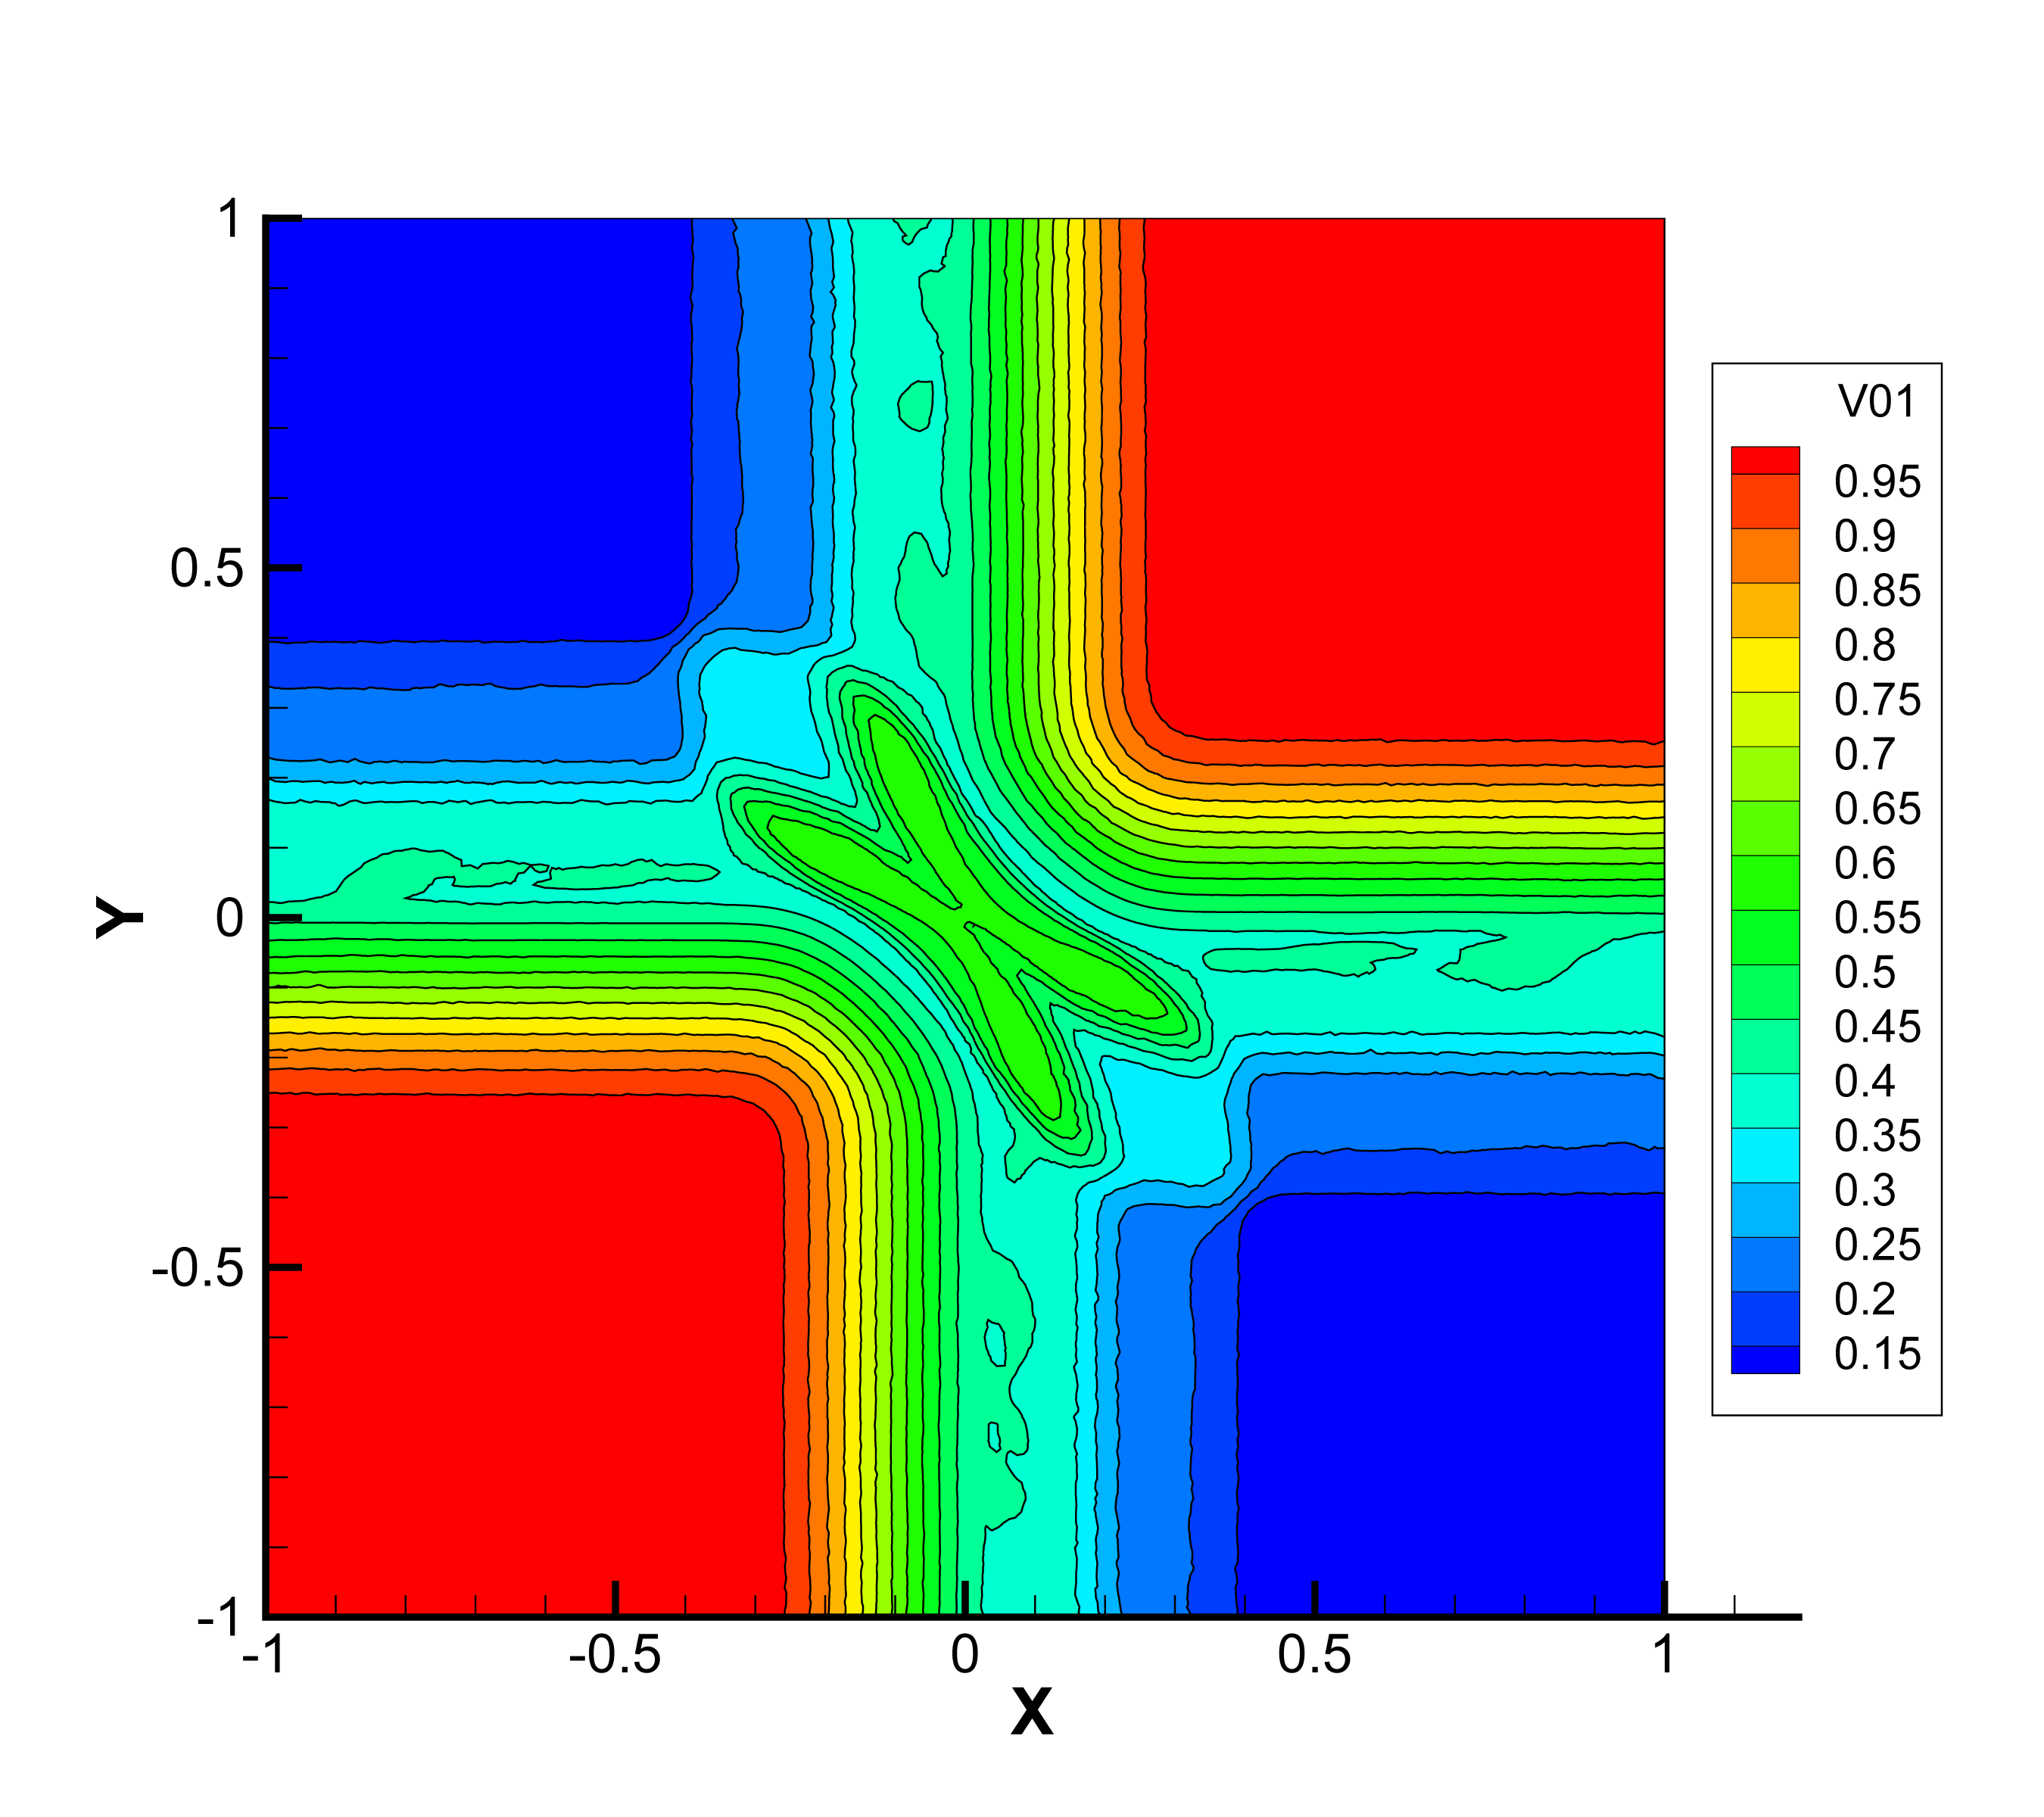
\includegraphics[width=0.6\columnwidth]{img/riemann2d_n.png}
	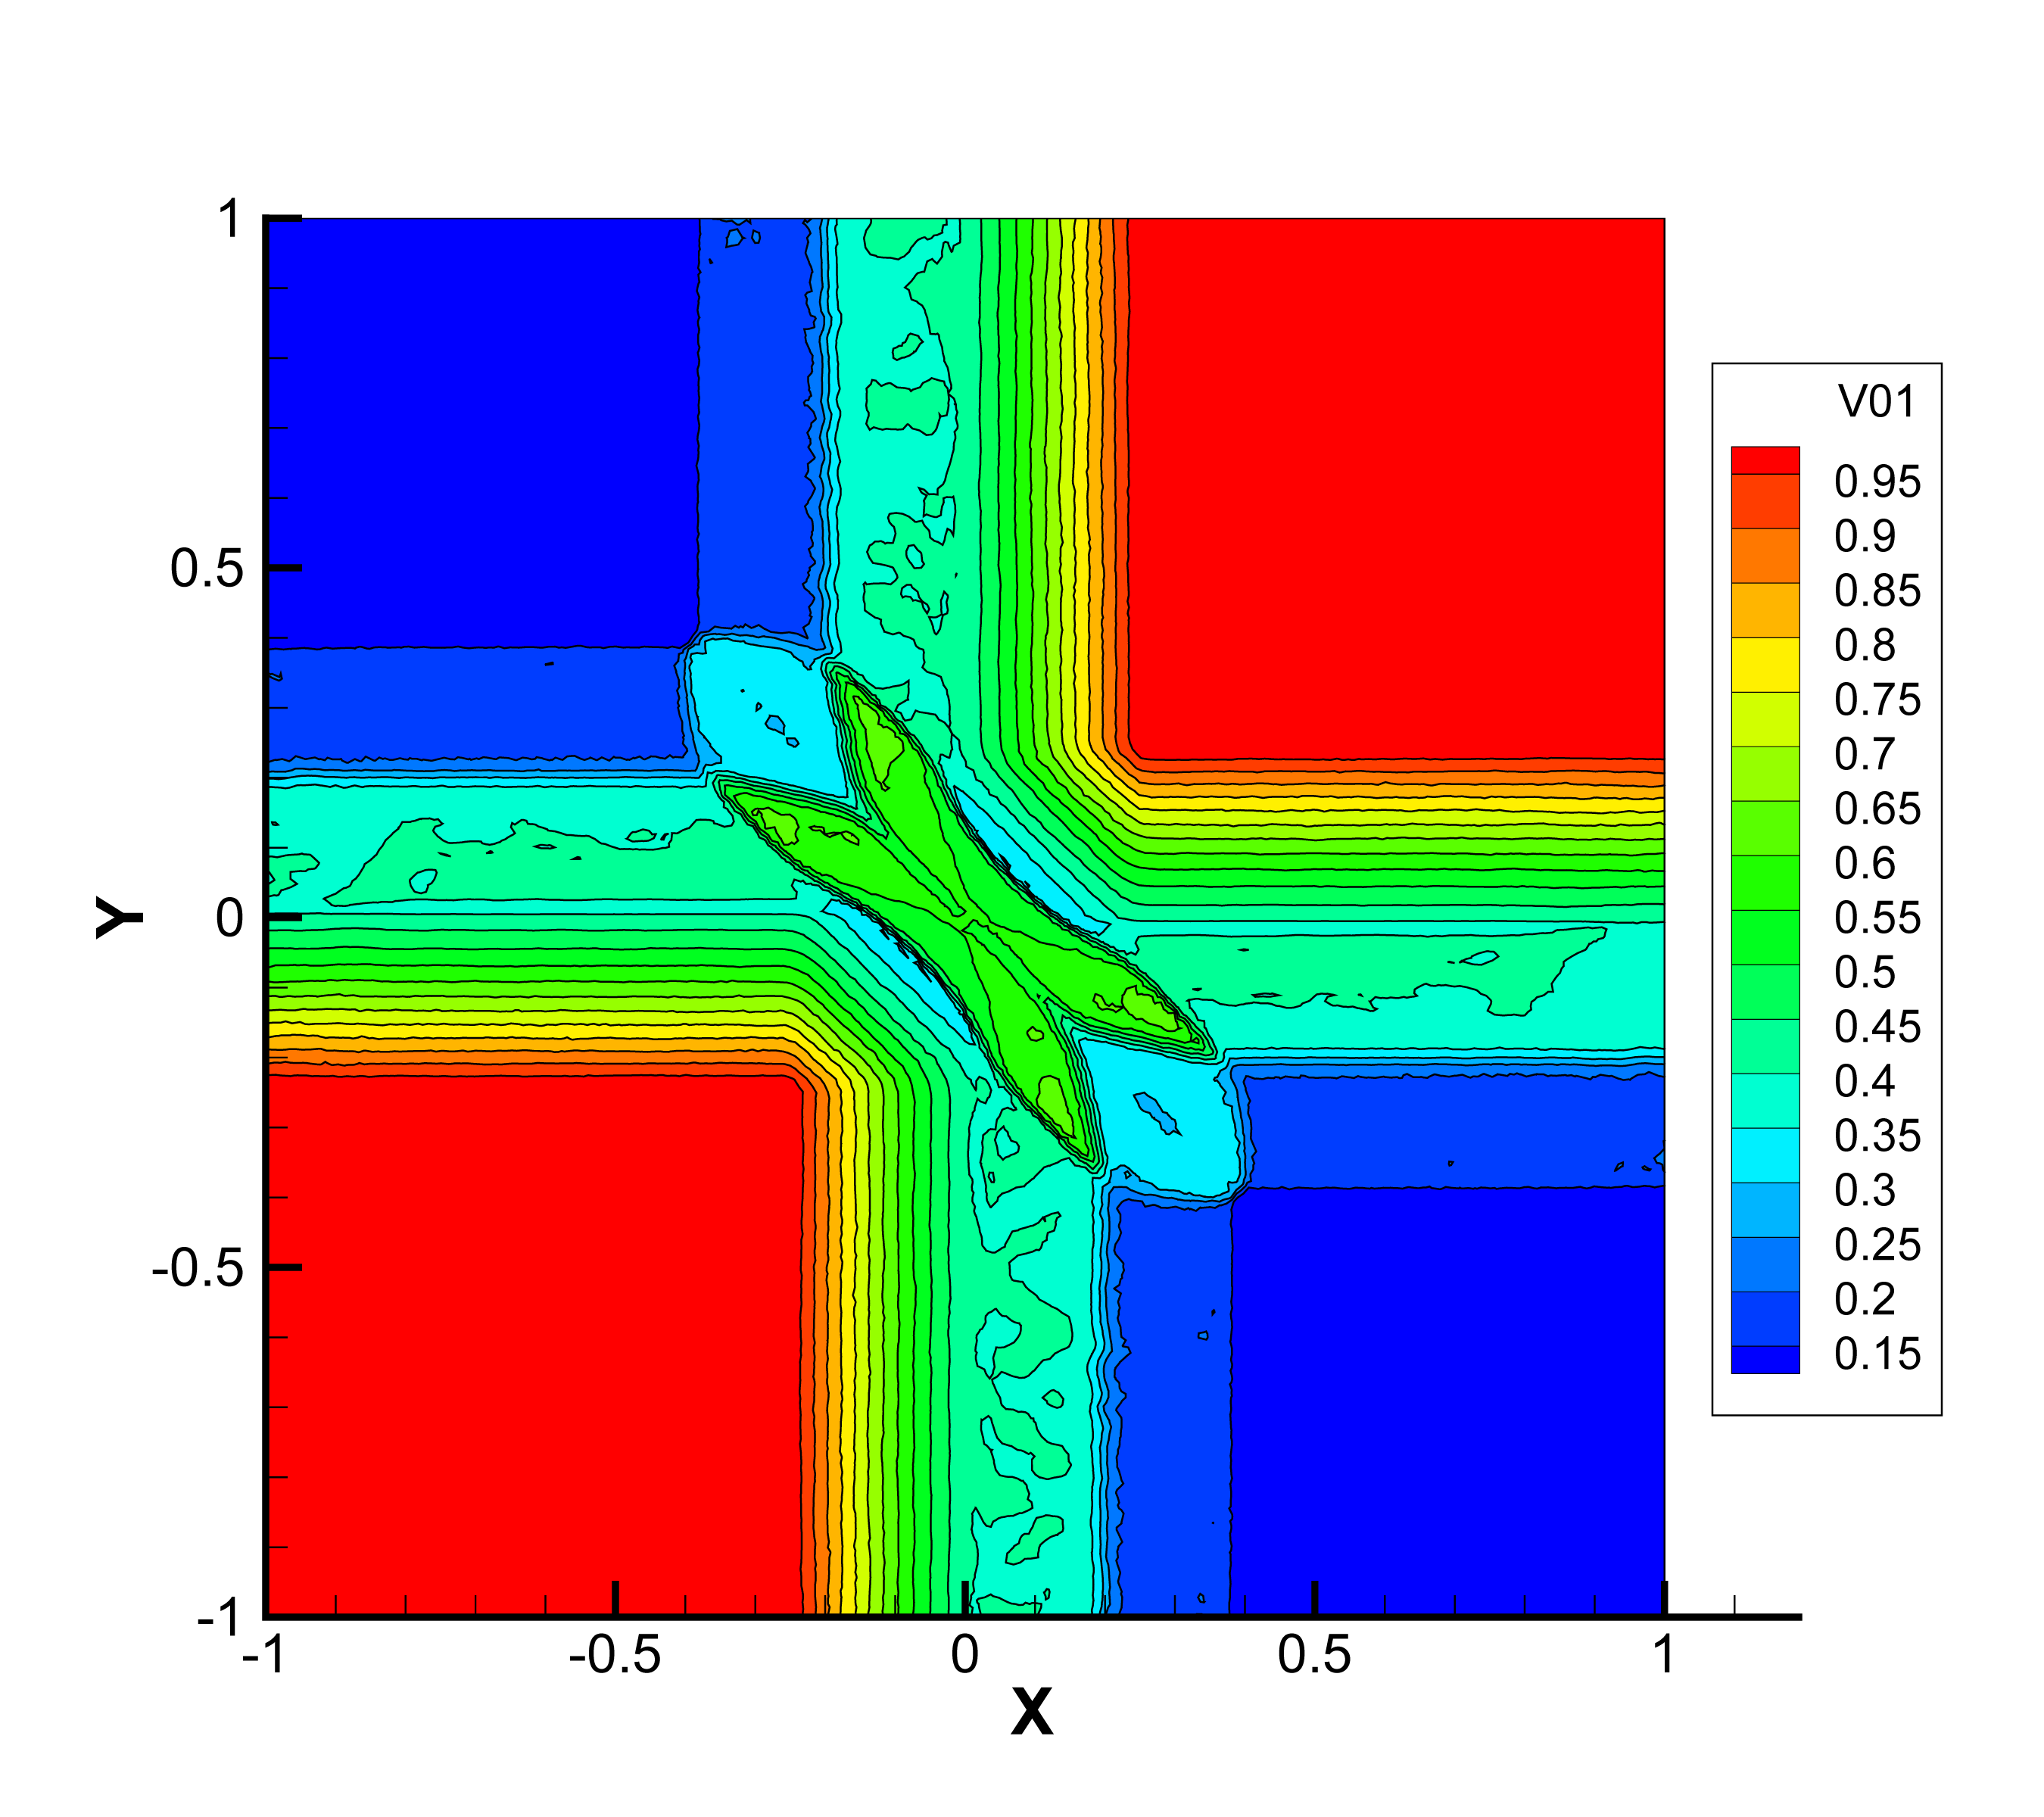
\includegraphics[width=0.6\columnwidth]{img/riemann2d_limn.png} \\
	\caption{2D Riemann -- final density field for N (top) and LimN (bottom) schemes}%
\end{figure}

\begin{figure}%
	\centering 
	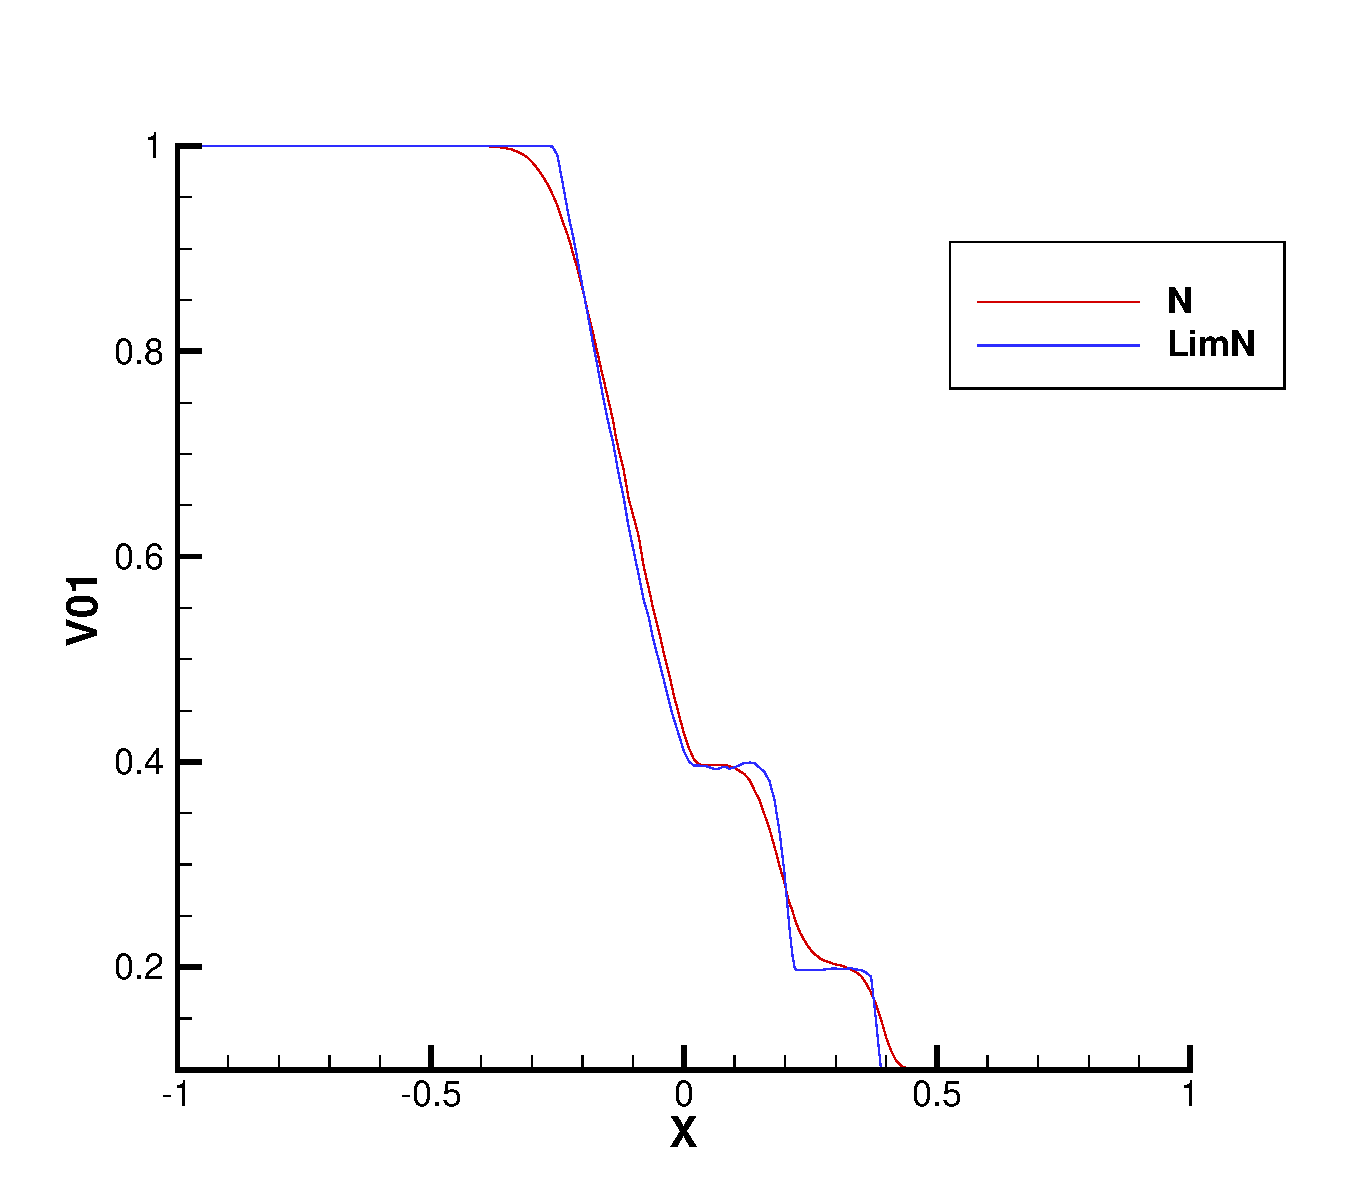
\includegraphics[width=0.6\columnwidth]{img/riemann2d_section.pdf} 
	\caption{2D Riemann -- final density field section at $y=-0.95$ }%
\end{figure}
\begin{enumerate}\addtocounter{enumi}{1}
	\item \begin{enumerate}\addtocounter{enumii}{1}
		\item \textbf{ Shock-shock interaction case: }
	\end{enumerate}
\end{enumerate}

This test case considers interaction of two discontinuities. Due to symmetry only upper half of domain was taken into account with appropriate boundary condition. Initial solution contains two discontinuities: normal shock at line $x=0.8$ and oblique at $y=0.8$ at the beginning. Arrows in figure points the direction of velocity. LimN and N schemes were considered. It can be seen that \rd{} method copes really well with complex structures in flow, even first order scheme. Limited N scheme offers better resolution of discontinuities in whole domain, which can be seen in figure containing density profile at symmetry line.


\begin{figure}%
	\centering
	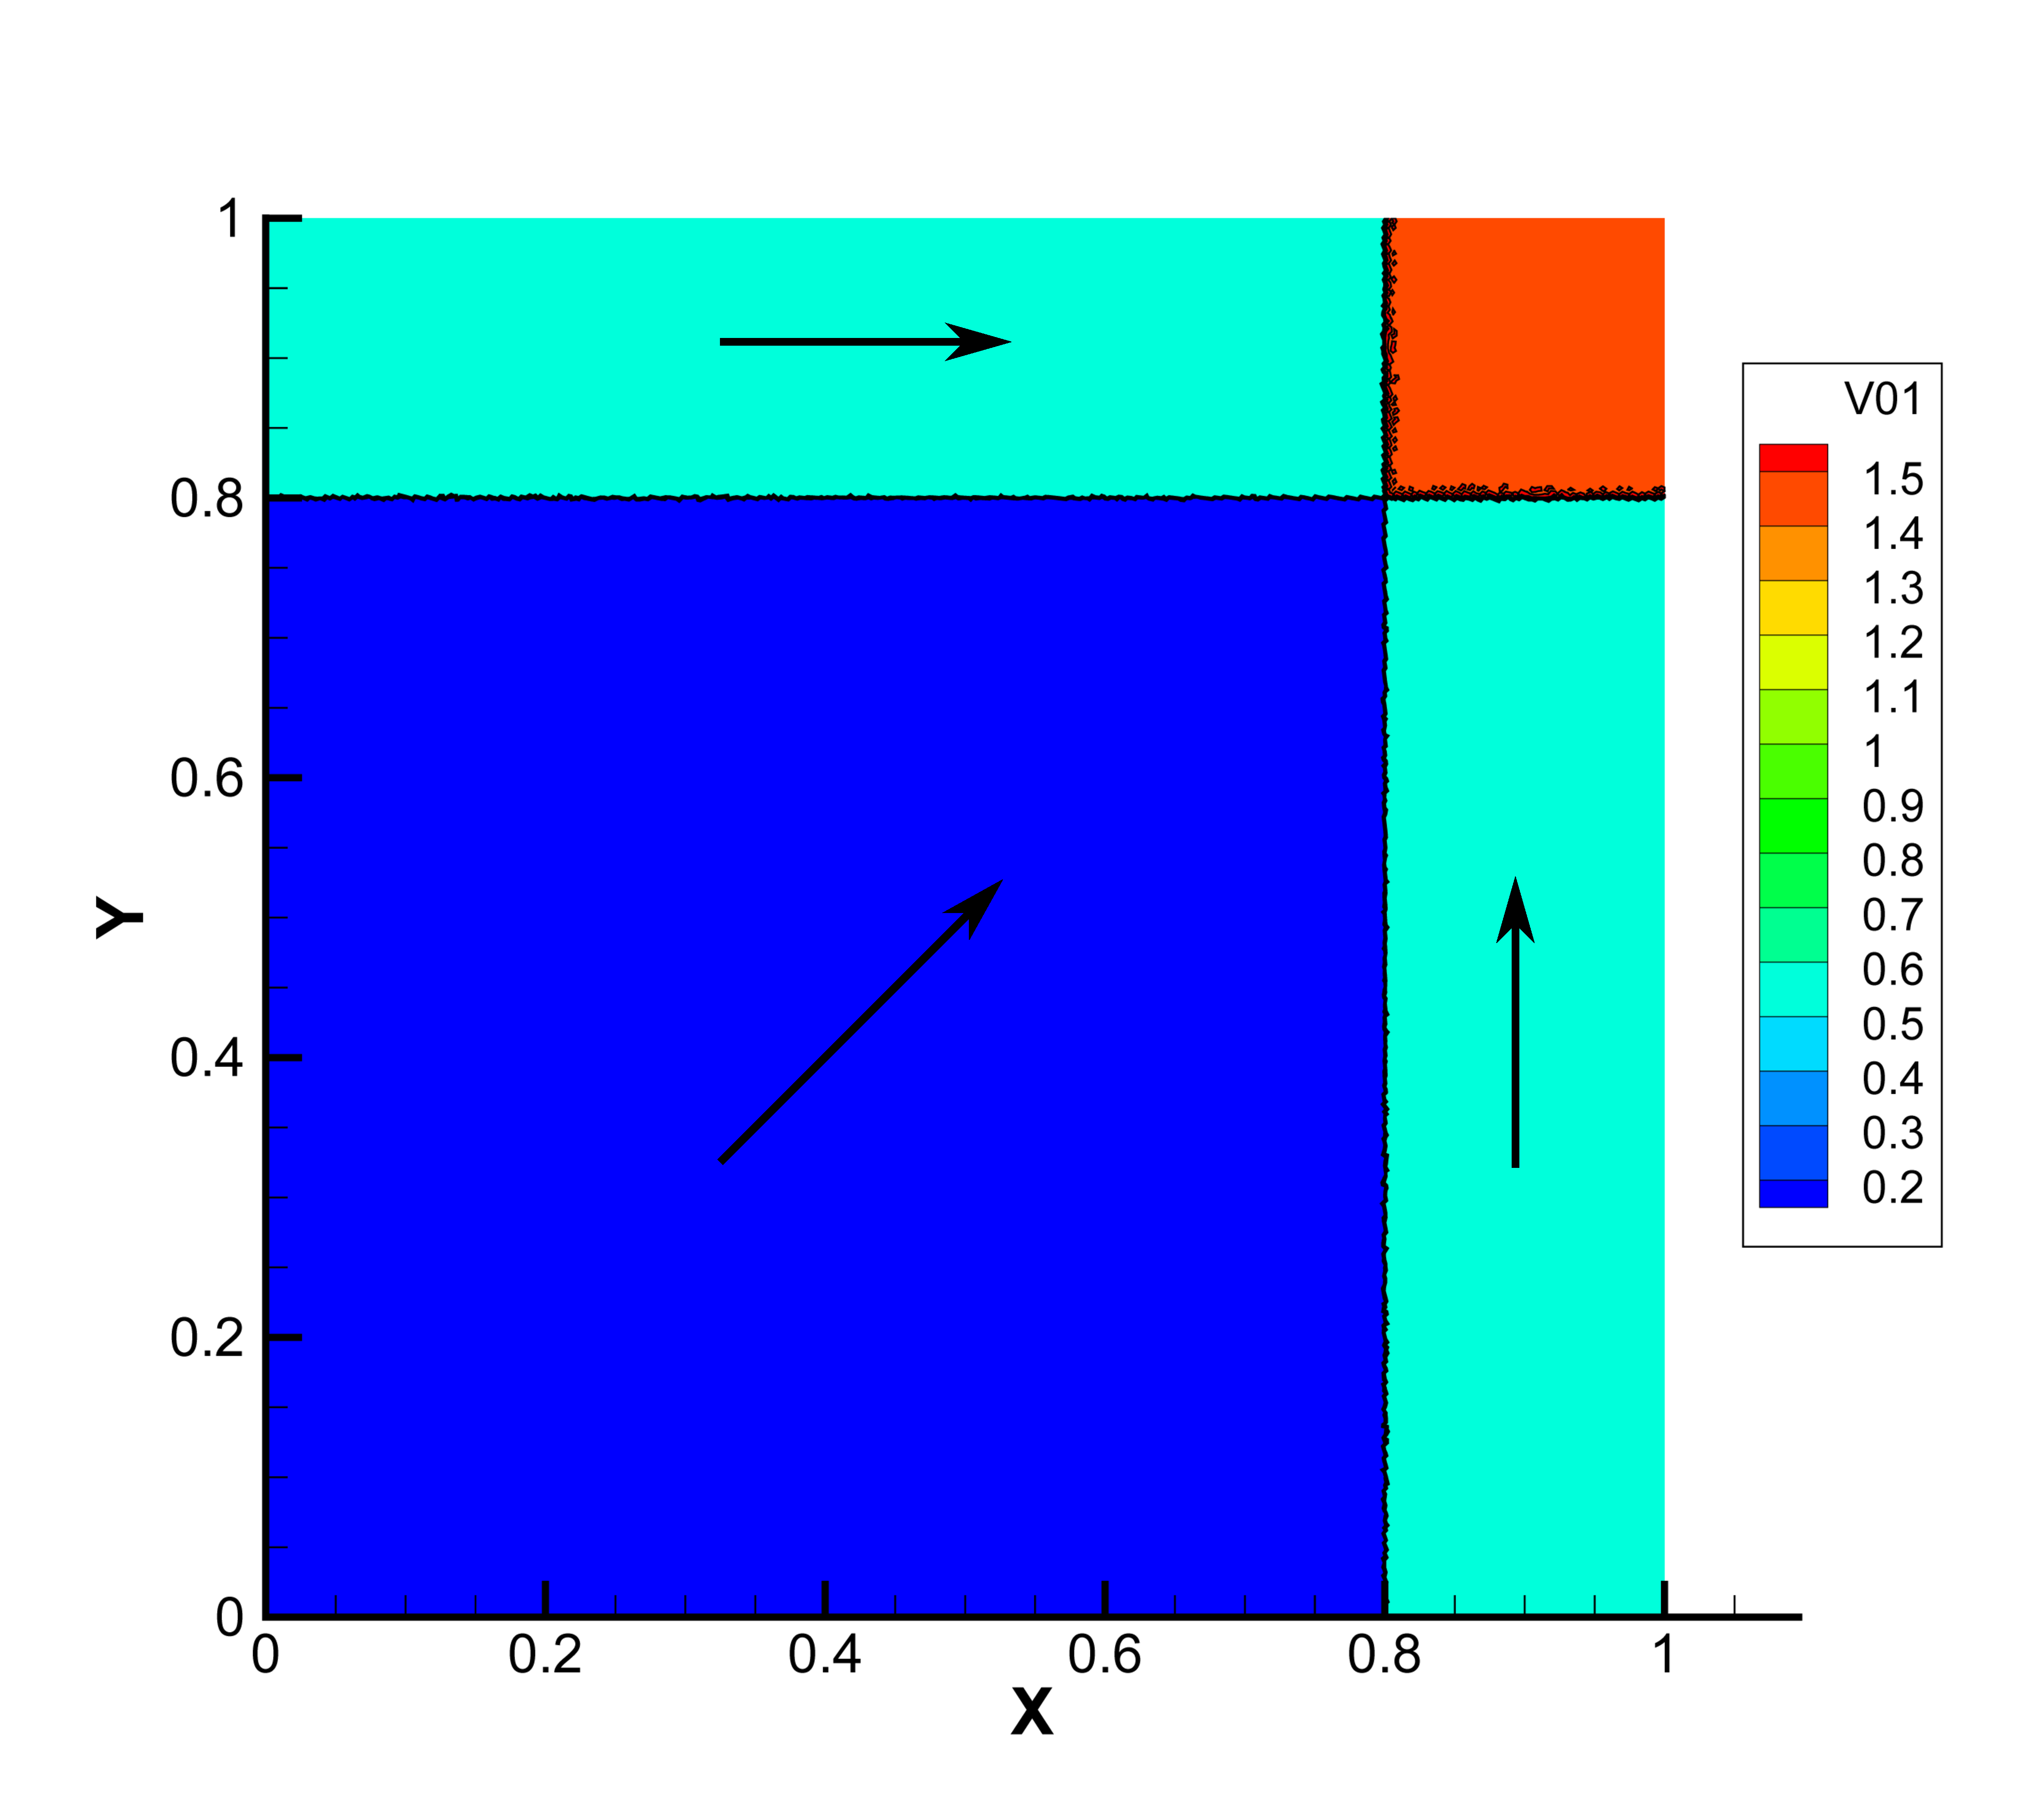
\includegraphics[width=0.65\columnwidth]{img/euler2shock_initial_ink.pdf}%
	\caption{Shock interaction -- initial solution}%
\end{figure}

\begin{figure}%
	\centering
	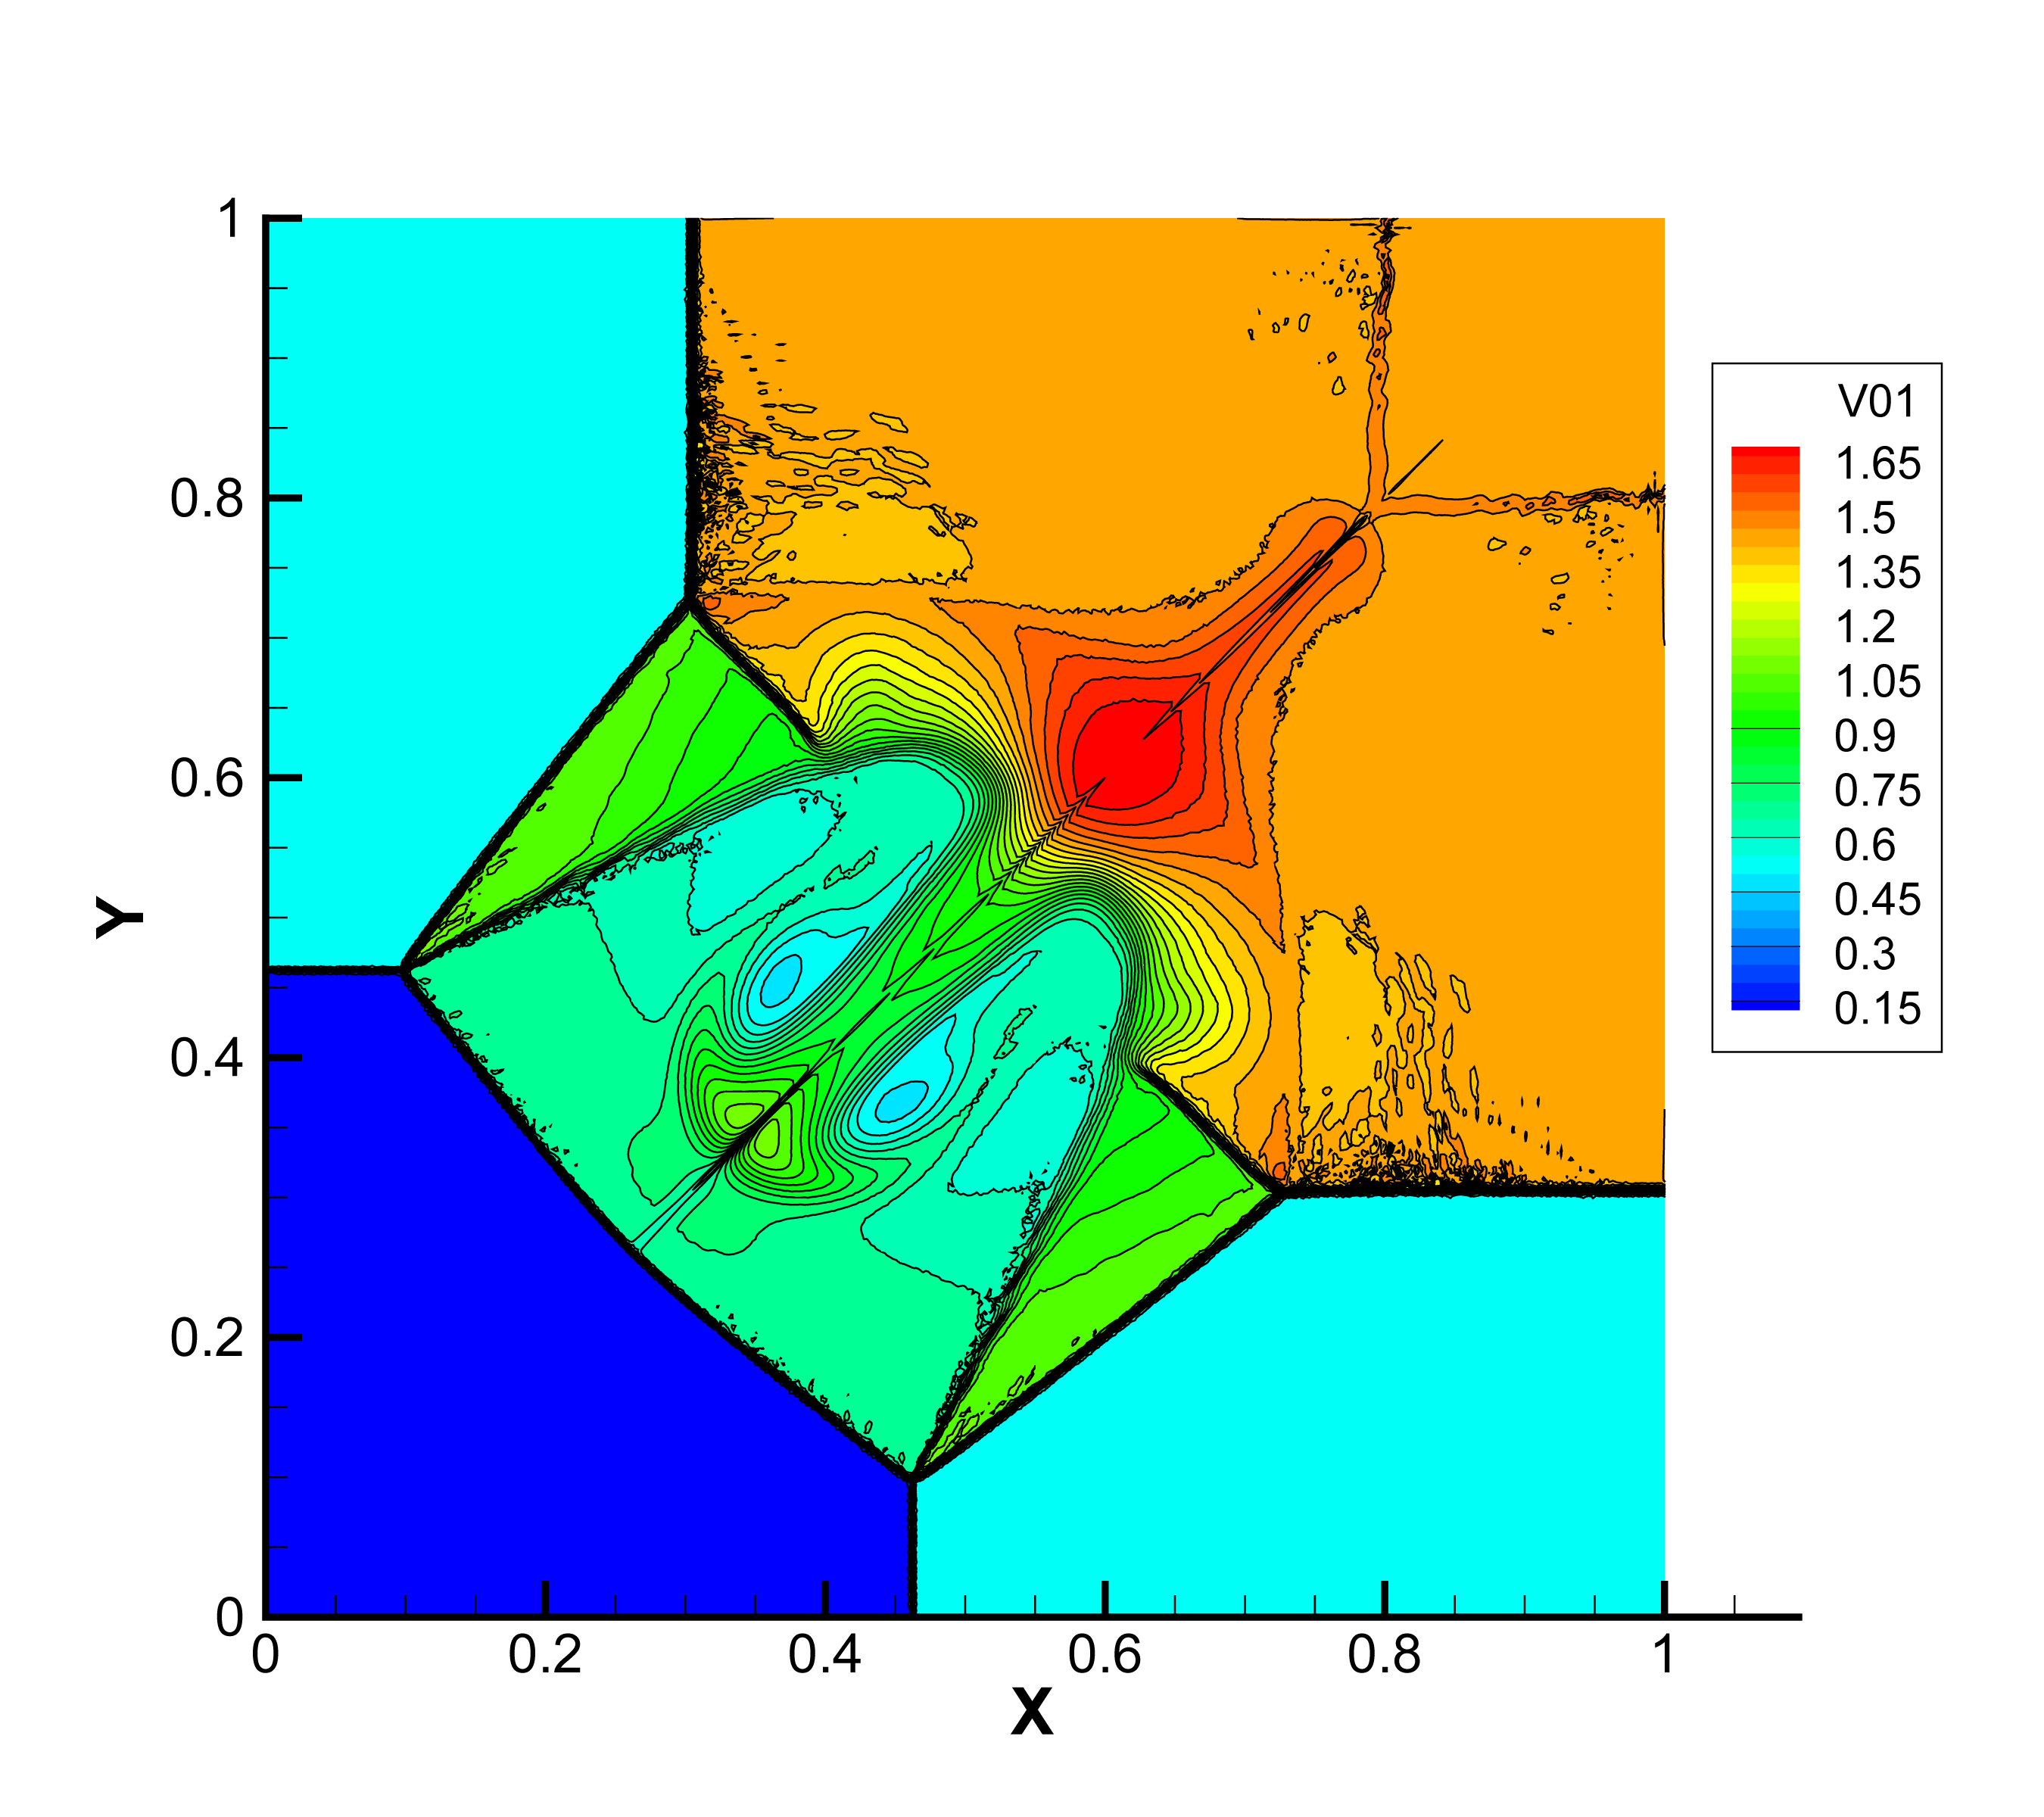
\includegraphics[width=0.65\columnwidth]{img/euler2shock_n.png} \\
	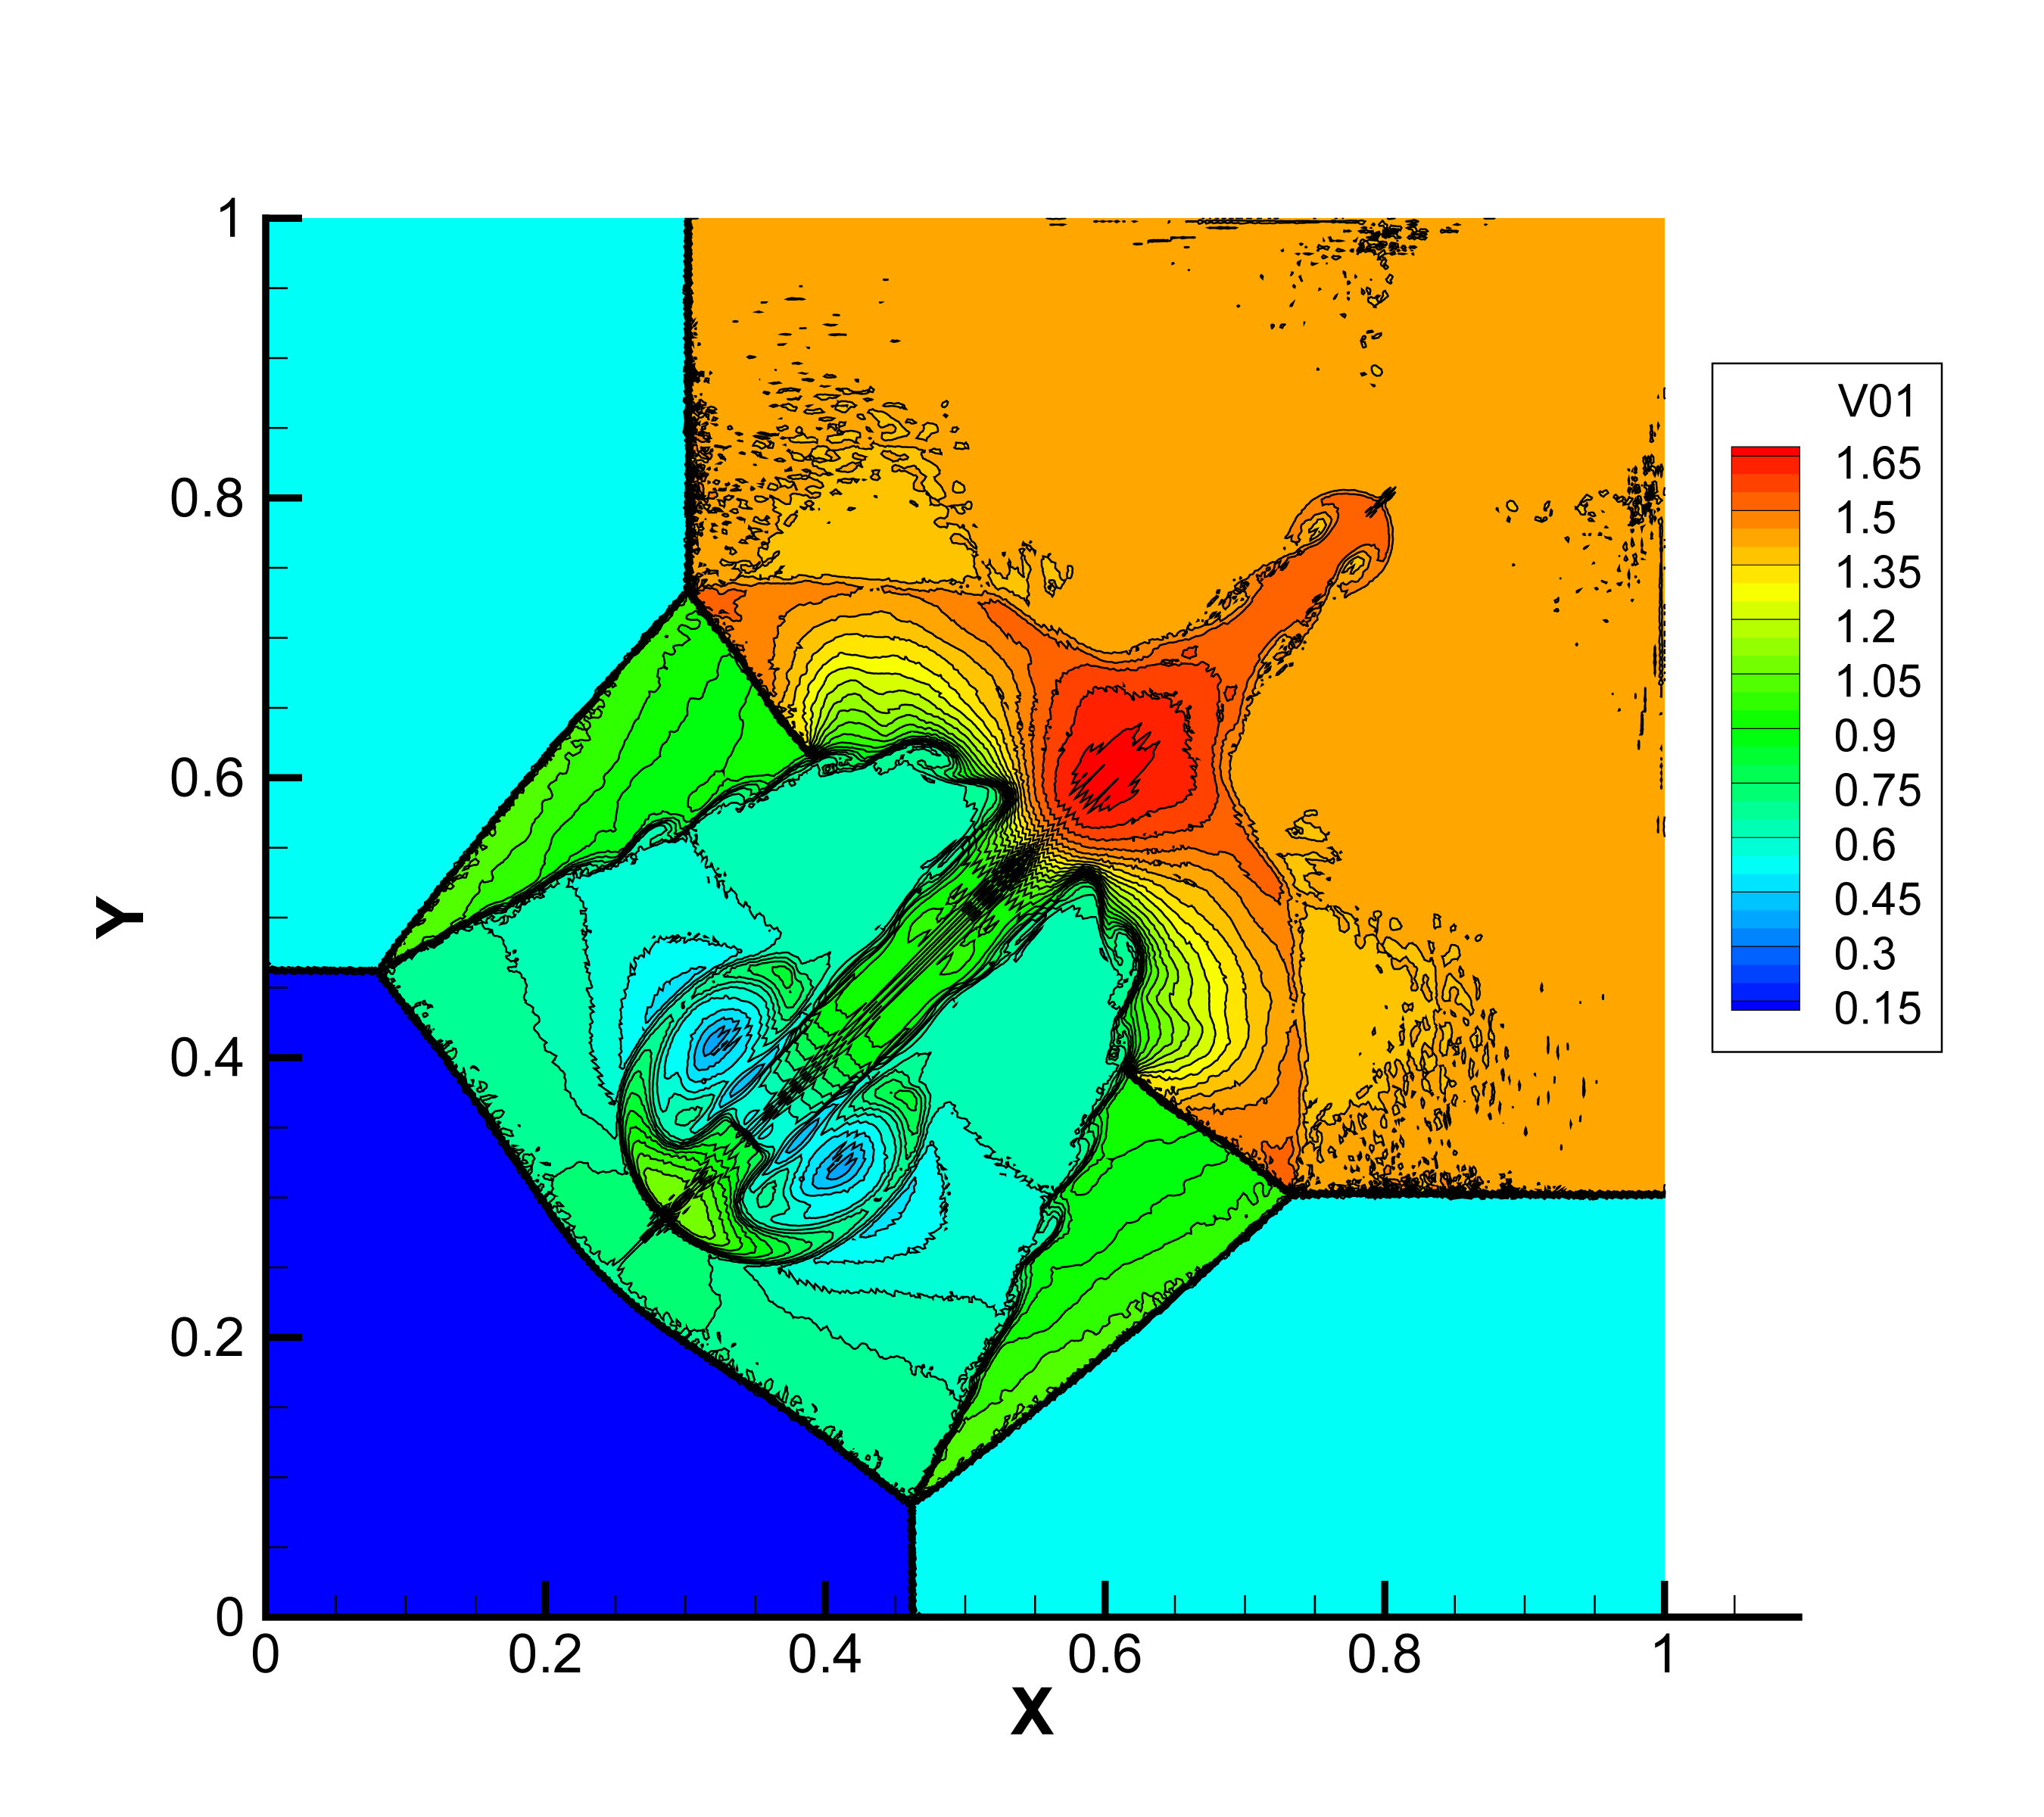
\includegraphics[width=0.65\columnwidth]{img/euler2shock_limn.png} \\
	\caption{Shock interaction -- final density field for N (left) and LimN (right) schemes}%
\end{figure}
\begin{figure}%
	\centering
	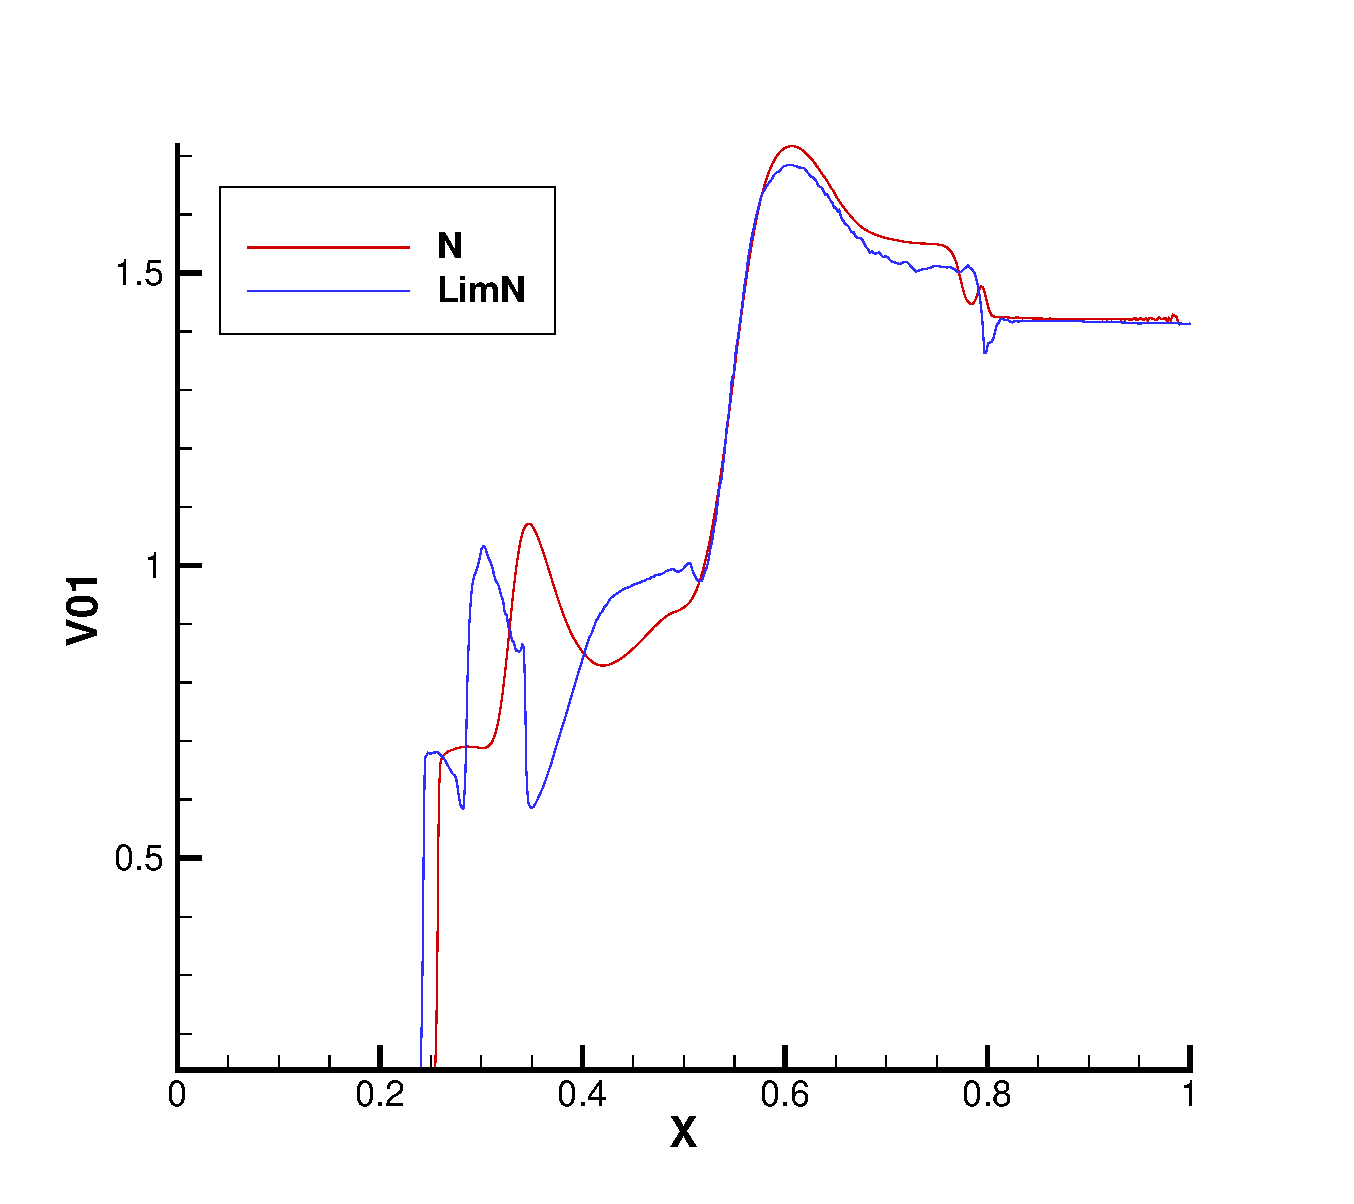
\includegraphics[width=0.65\columnwidth]{img/euler2shock_section.pdf} 
	\caption{Shock interaction -- final density field section at symmetry line}
	\label{}%
\end{figure}



\section{Conclusion}
Residual Distribution Method allows solving linear and general nonlinear hyperbolic systems in accurate, robust and efficient manner. Main advantage is that it can simulate complex flow structures, reaching second order of accuracy and satysfying monotonicity condition. Moreover, as it requires compact nearest-neighbour stencil, \rd{} is very easy to implement in parallel. Results presented here concerns only 2D test cases, but extension to 3D is straightforward. On the other hand, some issues are still open and requires further research, especially regarding nonlinear limited schemes.

\rd{} method was applied here for Euler equations, but there is possibilty to implement viscosity terms present in Navier-Stokes equations.

Residual Distribution Method has many important advantages compared to more mature FEM and FVM, and it can be thought as an alternative to these.


\end{multicols}


\end{document} 